\documentclass[conference]{IEEEtran}

% ---- Packages ----
\usepackage{amsmath,amssymb}
\usepackage{graphicx}
\usepackage{booktabs}
\usepackage[hidelinks]{hyperref}
\usepackage{tikz}
\usetikzlibrary{positioning,arrows.meta,shapes.multipart,fit,calc}

% ---- Title / Author (under the title only) ----
\title{SystemDK with AITL: Physics-Aware Runtime\\
DTCO via PID, FSM, and LLM Integration}

\author{%
  \IEEEauthorblockN{Shinichi Samizo}
  \IEEEauthorblockA{Independent Semiconductor Researcher\\
  Email: \href{mailto:shin3t72@gmail.com}{shin3t72@gmail.com}}
}

\begin{document}
\maketitle

\begin{abstract}
This paper presents SystemDK with AITL, a framework that extends conventional Design--Technology Co-Optimization (DTCO) by embedding control-theoretic loops directly into EDA flows. Compact PID controllers and FSM supervisors stabilize runtime variations (RC delay, thermal coupling, EMI/EMC disturbances). Future extensions (AITL Next) integrate LLM analyzers for adaptive PID retuning and FSM rule regeneration. The framework incorporates FEM analysis and S-parameter measurements into synthesis, P\&R, and STA, ensuring physics-aware closure. Simulations demonstrate order-of-magnitude improvements in timing stability, thermal robustness, and jitter suppression.
\end{abstract}

\begin{IEEEkeywords}
DTCO, CFET, PID control, FSM, LLM, EMI/EMC, thermal coupling, timing jitter, EDA.
\end{IEEEkeywords}

\section{Introduction}
Scaling to sub-2\,nm nodes and CFET integration introduces critical runtime effects:
\begin{itemize}
  \item RC delay variation due to interconnect scaling,
  \item Vertical thermal coupling in 3D-ICs,
  \item Stress-induced $V_\text{th}$ shifts,
  \item EMI/EMC noise degrading jitter and reliability.
\end{itemize}
Traditional DTCO applies static guardbands, leading to inefficiency. SystemDK with AITL proposes embedding runtime control (PID+FSM) and, in the future, LLM-based adaptation.

\section{Proposed Framework}
\subsection{AITL Base}
PID compensates delay/thermal/voltage variations; FSM supervises modes and safety thresholds.
\subsection{AITL Next}
A lightweight LLM analyzes EDA logs, retunes PID gains ($K_p,K_i,K_d$), and regenerates FSM rules.

% ===== Fig.1 (two-column, NOT under the title) =====
\begin{figure*}[t]
\centering
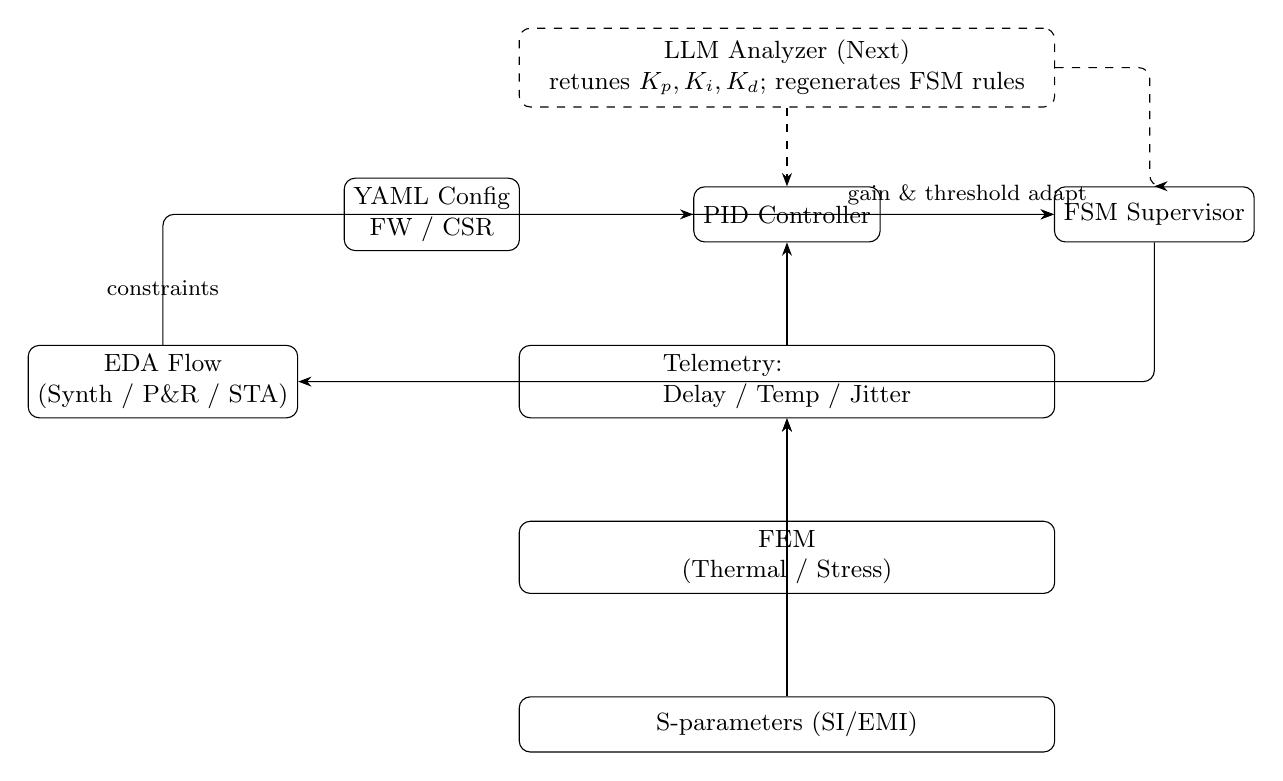
\begin{tikzpicture}[
  node distance=8mm, >=Stealth, rounded corners,
  font=\small,
  blk/.style={draw,rectangle,minimum width=22mm,minimum height=7mm,align=center}
]
% Top row
\node[blk] (yaml) {YAML Config\\FW / CSR};
\node[blk, right=22mm of yaml] (pid) {PID Controller};
\node[blk, right=22mm of pid] (fsm) {FSM Supervisor};

% Telemetry and physics stack
\node[blk, below=13mm of pid, minimum width=68mm, align=left] (tele)
      {Telemetry:\\Delay / Temp / Jitter};
\node[blk, below=13mm of tele, minimum width=68mm] (fem)
      {FEM\\(Thermal / Stress)};
\node[blk, below=13mm of fem, minimum width=68mm] (sparam)
      {S-parameters (SI/EMI)};

% EDA flow
\node[blk, left=28mm of tele] (eda) {EDA Flow\\(Synth / P\&R / STA)};

% Connections
\draw[->] (yaml) -- (pid);
\draw[->] (pid) -- node[above,font=\footnotesize]{gain \& threshold adapt} (fsm);
\draw[->] (tele) -- (pid);
\draw[->] (fem) -- (tele);
\draw[->] (sparam) -- (tele);
\draw[->] (eda) |- node[pos=.15,above,font=\footnotesize]{constraints} (fsm);
\draw[->] (fsm) |- (eda);

% LLM (future) -- dashed
\node[
  draw,dashed,rectangle,minimum width=68mm,minimum height=10mm,
  above=10mm of pid, align=center
] (llm) {LLM Analyzer (Next)\\retunes $K_p,K_i,K_d$; regenerates FSM rules};
\draw[->,dashed] (llm.south) -- (pid.north);
\draw[->,dashed] (llm.east) -- ++(12mm,0) |- (fsm.north);
\end{tikzpicture}
\caption{System overview (two-column): PID\,+\,FSM runtime control with telemetry; physics inputs (FEM, S-parameters); and an optional LLM analyzer for adaptive retuning.}
\label{fig:overview}
\end{figure*}
% ===== End Fig.1 =====

\section{Analytical Models and EDA Mapping}
\subsection{RC Delay Model}
\begin{equation}
t_{\mathrm{pd}}(T,\sigma,f)=R_0\!\left(1+\alpha_T (T-T_0)+\alpha_\sigma \sigma\right)C(f)+\Delta_{EMI}(f).
\end{equation}
Mapped to STA path-delay constraints.

\subsection{Thermal Coupling}
\begin{equation}
C_\mathrm{th}\,\frac{dT}{dt}+\frac{T-T_\mathrm{amb}}{R_\mathrm{th}}=P_\mathrm{chip}(t).
\end{equation}
Mapped to P\&R thermal placement constraints.

\subsection{Stress-Induced $V_{\text{th}}$ Shift}
\begin{equation}
\Delta V_\mathrm{th}(\sigma)=\kappa\cdot\sigma.
\end{equation}
Mapped to PDK/SPICE parameter updates.

\subsection{EMI Injection}
\begin{equation}
v_\mathrm{emi}(t)=A\sin(2\pi f_\mathrm{emi}t).
\end{equation}
Mapped to SI/EMC jitter constraints.

\section{Simulation Results with EDA Implications}

\subsection{RC Delay Compensation}
\begin{figure}[!t]
\centering
\includegraphics[width=.95\columnwidth]{figs/sim_delay_rc.png}
\caption{RC delay variation normalized (Uncontrolled, PID, PID+FSM).}
\label{fig:rc}
\end{figure}

\subsection{Thermal Response Control}
\begin{figure}[!t]
\centering
\includegraphics[width=.95\columnwidth]{figs/sim_thermal_response.png}
\caption{Thermal response $\Delta T$ reduction with PID and PID+FSM.}
\label{fig:thermal}
\end{figure}

\subsection{EMI Jitter Suppression}
\begin{figure}[!t]
\centering
\includegraphics[width=.95\columnwidth]{figs/sim_emi_jitter.png}
\caption{Jitter reduction under injected EMI.}
\label{fig:emi}
\end{figure}

\subsection{FEM Analysis}
\begin{figure}[!t]
\centering
\includegraphics[width=.95\columnwidth]{figs/fem_thermal_map.png}\\[2mm]
\includegraphics[width=.95\columnwidth]{figs/fem_stress_map.png}
\caption{FEM maps: thermal hotspot (top) and TSV-induced stress (bottom).}
\label{fig:fem}
\end{figure}

\subsection{S-Parameter Analysis}
\begin{figure}[!t]
\centering
\includegraphics[width=.95\columnwidth]{figs/sparam_s11s21.png}
\caption{S11/S21 trends under control states.}
\label{fig:sparam}
\end{figure}

\section{Implementation PoC}
RTL excerpt (PID controller), FSM transitions, and YAML configuration were implemented in Verilog and integrated with APB/AXI-Lite CSRs.

\section{Discussion}
\begin{itemize}
\item Guardbands $\rightarrow$ adaptive loops,
\item Static sign-off $\rightarrow$ dynamic runtime closure,
\item Reliability $\rightarrow$ cross-domain resilience (delay, thermal, stress, EMI).
\end{itemize}

\section{Conclusion and Future Work}
AITL Base (PID\,+\,FSM) establishes runtime stabilization. AITL Next will integrate lightweight LLM models for real-time EDA log analysis and control redesign. Industrial relevance: prototype chips, EDA tool collaboration, and AI-driven DTCO.

% ---------- References (manual) ----------
\begin{thebibliography}{6}
\bibitem{yakimets2020}
D.~Yakimets \emph{et al.}, ``Challenges for cfet integration,'' in \emph{Proc. IEEE IEDM}, 2020, pp. 19.1.1--19.1.4.
\bibitem{irds2023}
IRDS, ``International roadmap for devices and systems (irds) 2023,'' 2023. [Online]. Available: \url{https://irds.ieee.org/roadmap-2023}
\bibitem{franklin2002}
G.~Franklin, J.~D. Powell, and A.~Emami-Naeini, \emph{Feedback Control of Dynamic Systems}, 7th ed. Pearson, 2015.
\bibitem{khalil2002}
H.~K. Khalil, \emph{Nonlinear Systems}. Prentice Hall, 2002.
\bibitem{anderson2007}
B.~D.~O. Anderson and J.~B. Moore, \emph{Optimal Control: Linear Quadratic Methods}. Dover, 2007.
\bibitem{iec61967}
IEC, \emph{Electromagnetic Compatibility (EMC) --- Part 4: Testing and Measurement Techniques}, IEC Std. 610 00-4, 2019.
\end{thebibliography}

% ---------- Author Biography (classic IEEEtran style, no photo, 1 author) ----------
\section*{Author Biography}
\noindent\textbf{Shinichi Samizo}
received the M.S. degree in Electrical and Electronic Engineering from Shinshu University, Japan. He worked at Seiko~Epson Corporation as an engineer in semiconductor memory and mixed-signal device development, and also contributed to inkjet MEMS actuators and PrecisionCore printhead technology. He is currently an independent semiconductor researcher focusing on process/device education, memory architecture, and AI system integration. \textbf{Contact:} \href{mailto:shin3t72@gmail.com}{shin3t72@gmail.com}, \href{https://github.com/Samizo-AITL}{Samizo-AITL}.
\end{document}
